\documentclass{beamer}
\usetheme{Darmstadt}
\usecolortheme{beaver}
\usepackage{listings}
\usepackage[utf8]{inputenc}
\usepackage[french]{babel}


\begin{document}

\author{Rémy \textsc{El Sibaïe Besognet}}
\title{OCaml pour la combinatoire}
\date{\today}

\begin{frame}
  \titlepage
\end{frame}

%%% 1 EMC
\begin{frame}{Exact Matrix Covering}

Problème EMC ou couverture exacte de matrice :


 \begin{columns}

    \column{0.5\textwidth}
				\begin{itemize}
				\item Un sous ensemble de lignes avec un et un seul 1 par colonne
				\item Série de contraintes
				\item pas d'algorithme efficace
				\end{itemize}

    \column{0.5\textwidth}
  \begin{displaymath}
   \left(\begin{array}{ c c c c c }
   1 & 0 & 1 & 1 \\
   0 & 1 & 1 & 0 \\
   1 & 1 & 0 & 1 \\
   1 & 0 & 0 & 1 \\
   0 & 1 & 0 & 0
  \end{array}\right)
  \end{displaymath}

  \end{columns}
\end{frame}


\begin{frame}{EMC : exemple}

\begin{displaymath}
   \left(\begin{array}{ c c c c c }
   1 & 0 & 1 & 1 \\
   0 & 1 & 1 & 0 \\
   1 & 1 & 0 & 1 \\
   1 & 0 & 0 & 1 \\
   0 & 1 & 0 & 0
  \end{array}\right)
  \end{displaymath}

\begin{center}
$ \{3, 4\} $ n'est pas une solution\\
$ \{0, 4\}, \{1, 3\} $ sont des solutions
\end{center}
\end{frame}

\begin{frame}{Application : Pavage}
\[
  \begin{array}{|c|c|c|c|}
		\hline
   	0 & 1 & 2 & 3 \\
		\hline
    4	& 5 & 6 & 7 \\
		\hline
   	8 & 9 & 10 & 11 \\
		\hline
   	12 & 13 & 14 & 15 \\
		\hline
\end{array}
	\textrm{ }
\begin{array}{ |c| }
	\hline
		\\
	\hline
    \\
	\hline
  \end{array}
	\textrm{ }
\begin{array}{ |c|c| }
	\hline
		& \\ 
	\hline
  \end{array}
\]
Poser un domino sur la case 0 :
\[
  \begin{array}{ c c c c c c c c c c c c c c c c }
	1 & 1 & 0 & 0 & 0 & 0 & 0 & 0 & 0 & 0 & 0 & 0 & 0 & 0 & 0 & 0 
  \end{array}
\]
\end{frame}



\begin{frame}{Application : Sudoku}

\begin{figure}[h]
\scalebox{0.7}{
\centering

$\begin{array}{|c|c|c||c|c|c||c|c|c|}
\hline
5 & 3 &   &   & 7 &   &  &   &    \\
\hline
6 &   &   & 1 & 9 & 5 &  &   &    \\
\hline
  & 9 & 8 &   &   &   &  & 6 &    \\
\hline
\hline
8 &   &   &   & 6 &   &   &   & 3 \\
\hline
4 &   &   & 8 &   & 3 &   &   & 1 \\
\hline
7 &   &   &   & 2 &   &   &   & 6 \\
\hline
\hline
  & 6 &   &   &   &   & 2 & 8 &   \\
\hline
  &   &   & 4 & 1 & 9 &   &   & 9 \\
\hline
  &   &   &   & 8 &   &   & 7 & 5 \\
\hline
\end{array}$
}
\end{figure}

4 contraintes : 
\begin{itemize}
\item la case (l'espace)
\item la ligne (la valeur)
\item la colonne (la valeur)
\item la cellule 3x3 (la valeur)
\end{itemize}
\end{frame}





\begin{frame}{Application : N-Reines}
\begin{figure}[h]
\begin{center}
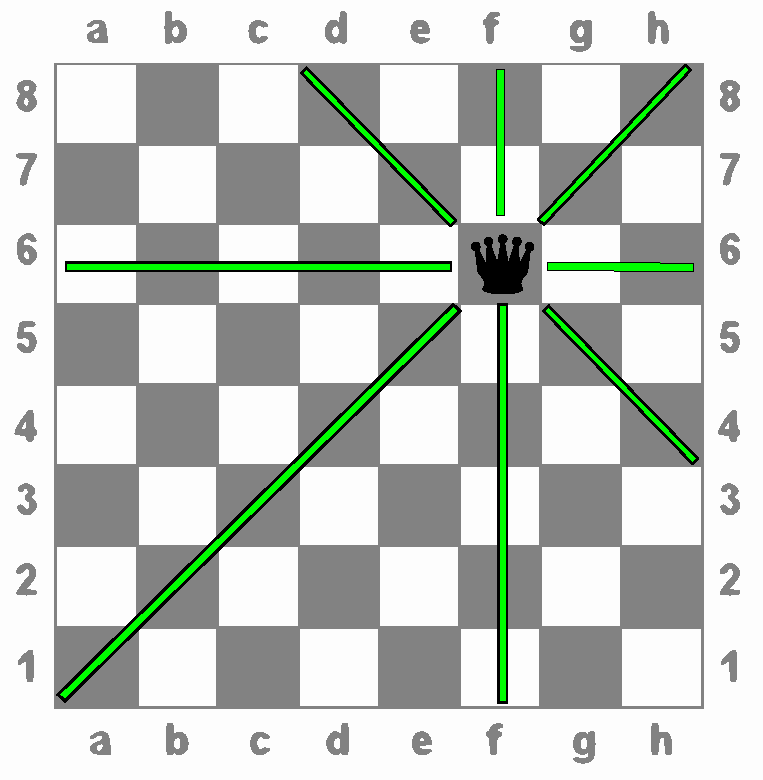
\includegraphics[height=0.4\textheight]{../imports/8queens.pdf}
\end{center}
\end{figure}

4 contraintes : 
\begin{itemize}
\item la ligne
\item la colonne
\item la diagonale gauche-droite
\item la diagonale droite-gauche
\end{itemize}

\end{frame}


%%% 2 DLX
\begin{frame}{Résoudre EMC : Le Dancing Links de Knuth}

The Dancing Links, Les liens dansants, ou DLX\\
Un principe astucieux des listes doublements chaînées : 
\begin{figure}[h]
\begin{center}
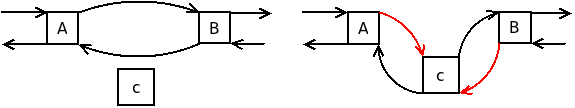
\includegraphics[scale=0.5]{../imports/add_elmt_dll.png}
\end{center}
\end{figure}
Ajouter un élément : évident.
\end{frame}

\begin{frame}{Principe de base de DLX}
Plus élégant : Suppression puis ré-ajout
\begin{figure}[h]
\begin{center}
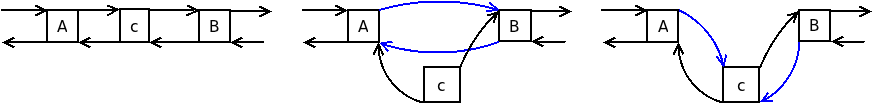
\includegraphics[scale=0.3]{../imports/delete.png}
\end{center}
\end{figure}
\end{frame}

\begin{frame}{Une structure exotique}

La matrice doublement chaînée

 \begin{columns}
    \column{0.5\textwidth}
\begin{center}$
\left(\begin{array}{ c c c c c }
   1 & 1 \\
   0 & 1 
  \end{array}\right)$
\end{center}

    \column{0.5\textwidth}
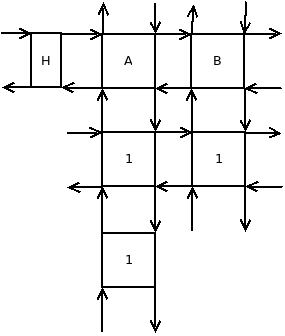
\includegraphics[scale=0.4]{../imports/dlx_matrice.png}
 \end{columns}

Présence d'en-têtes, circulaire, contient uniquement les 1 de EMC.
\end{frame}


\begin{frame}{Structure en OCaml}
\scalebox{0.8}{
\lstinputlisting[language=Caml]{../imports/node.ml}
}
\end{frame}

\begin{frame}{L'algorithme X}
\scalebox{0.6}{
\lstinputlisting[language=Caml]{../imports/search.ml}
}
\end{frame}



%%% 3 ZDD
\begin{frame}{Zero-Suppressed Binary Decision Diagram}
Un type de Diagramme de Décision Binaire (BDD)\\
Surnom : ZDD
\begin{itemize}
\item Arbre binaire avec des propriétés
\item Ensemble d'ensemble d'entiers
\item Structure optimisée pour EMC
\end{itemize}
\end{frame}

\begin{frame}{ZDD : Definition}
\begin{figure}[htp]
\begin{center}
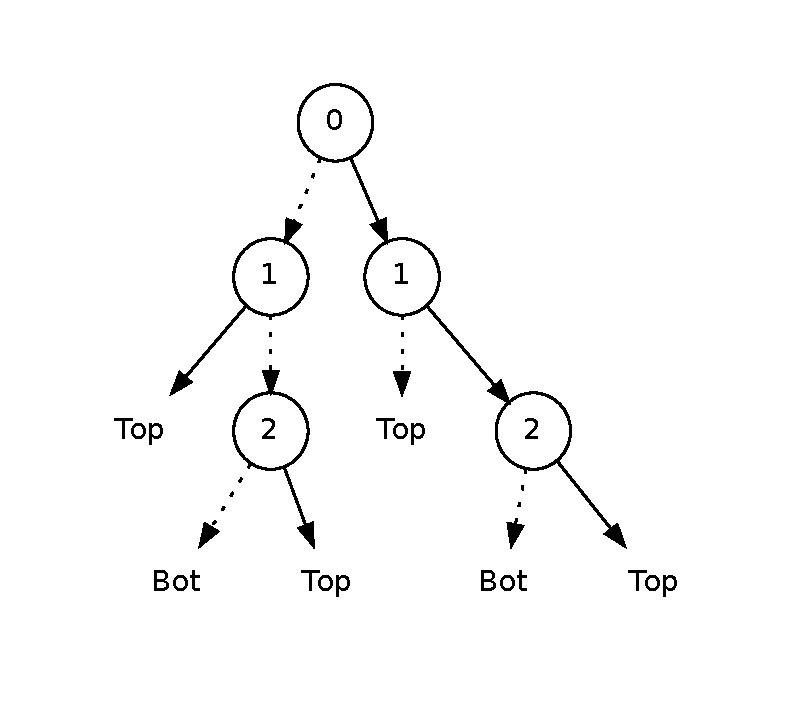
\includegraphics[scale=0.3]{../imports/zdd_ex.pdf}
\end{center}
\end{figure}
\begin{itemize}
\item Feuilles : $\bot$ (Bottom) ou $\top$ (Top)
\item Pas de $\bot$ à droite
\item Un n\oe ud : i $\rightarrow$ $L$, $R$ tel
que L et R ne contiennent pas d'élément j avec j $\leq$ i \\
\end{itemize} 
\end{frame}


\begin{frame}{ZDD : Un ensemble d'ensemble}
Sur l'ensemble $E = \{0, 1,..,n\}$
\begin{figure}[htp]
\begin{center}
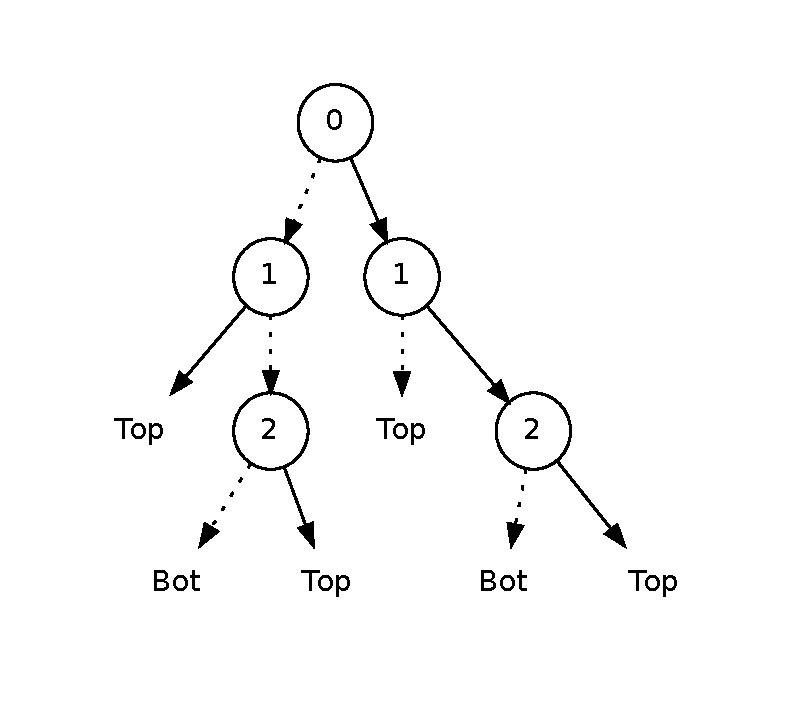
\includegraphics[scale=0.3]{../imports/zdd_ex.pdf}
\end{center}
\end{figure}
correspond à \{\{0, 1, 2\}, \{0\}, \{1\}, \{2\}\}
\end{frame}


\begin{frame}{ZDD : Optimisations}
Economie sur la mémoire et le temps (construction et parcourt)
\begin{center}
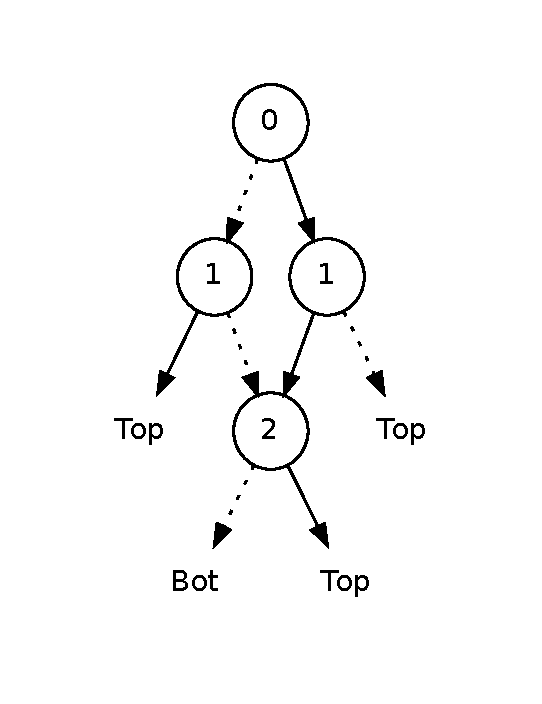
\includegraphics[scale=0.4]{../imports/zdd_construct.pdf}
\end{center}

grâce à : \emph{mémoïzation} et \emph{hash consing}

\end{frame}

\begin{frame}{Réduction vers EMC : une colonne}
  \begin{columns}
    \column{0.5\textwidth}

  \begin{displaymath}
   \left(\begin{array}{ c c c c c }
   1 & 0 & 1 & 1 \\
   0 & 1 & 1 & 0 \\
   1 & 1 & 0 & 1 \\
   1 & 0 & 0 & 1 \\
   0 & 1 & 0 & 0
  \end{array}\right)
  \end{displaymath}

    \column{0.5\textwidth}
    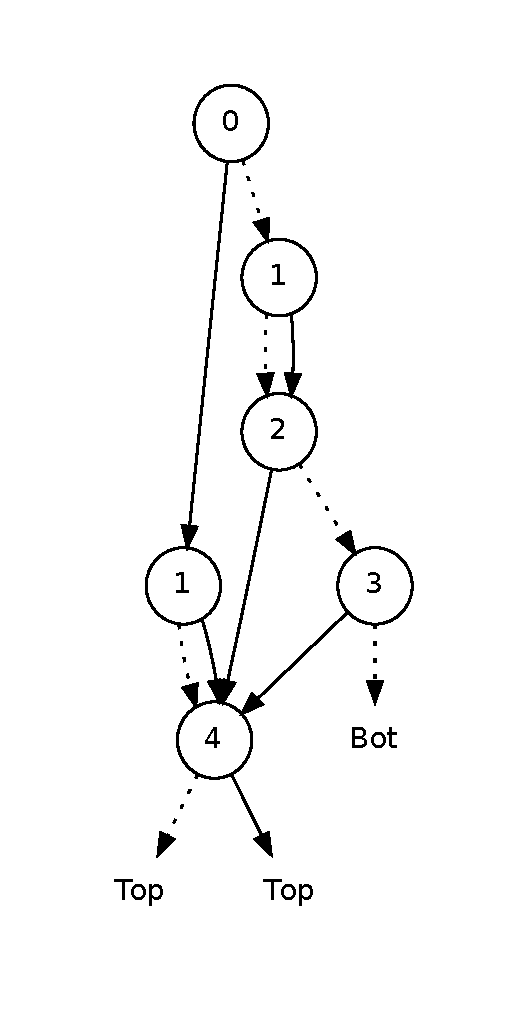
\includegraphics[height=0.9\textheight]{../imports/column.pdf}
  \end{columns}
\end{frame}

\begin{frame}{Réduction vers EMC : après intersection}
  \begin{columns}
    \column{0.3\textwidth}

  \begin{displaymath}
   \left(\begin{array}{ c c c c c }
   1 & 0 & 1 & 1 \\
   0 & 1 & 1 & 0 \\
   1 & 1 & 0 & 1 \\
   1 & 0 & 0 & 1 \\
   0 & 1 & 0 & 0
  \end{array}\right)
  \end{displaymath}

    \column{0.7\textwidth}
    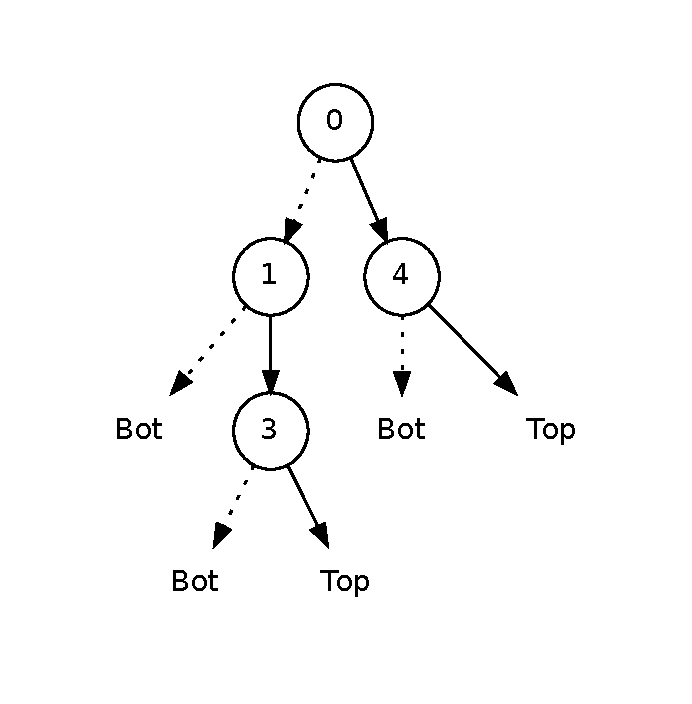
\includegraphics[height=0.8\textheight]{../imports/inter.pdf}
  \end{columns}
\end{frame}

\begin{frame}{}
\begin{center}
    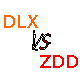
\includegraphics[height=0.5\textheight]{../imports/vs.pdf}
\end{center}
DLX : avantage en mémoire, n'est pas dépendant de la matrice EMC\\
ZDD : avantage en temps (très puissant), fait exploser la mémoire \\
Conclusion : égalité
\end{frame}



%%% 4 bibliothèque OCaml
\begin{frame}{ReMl : une bibliothèque OCaml}
\begin{itemize}
\item Outils pour résoudre EMC
\item Outils pour encoder dans EMC
\item Un mini langage pour le pavage
\end{itemize}
\end{frame}


\begin{frame}{ReMl : Architecture des modules}
\begin{figure}[htp]
\begin{center}
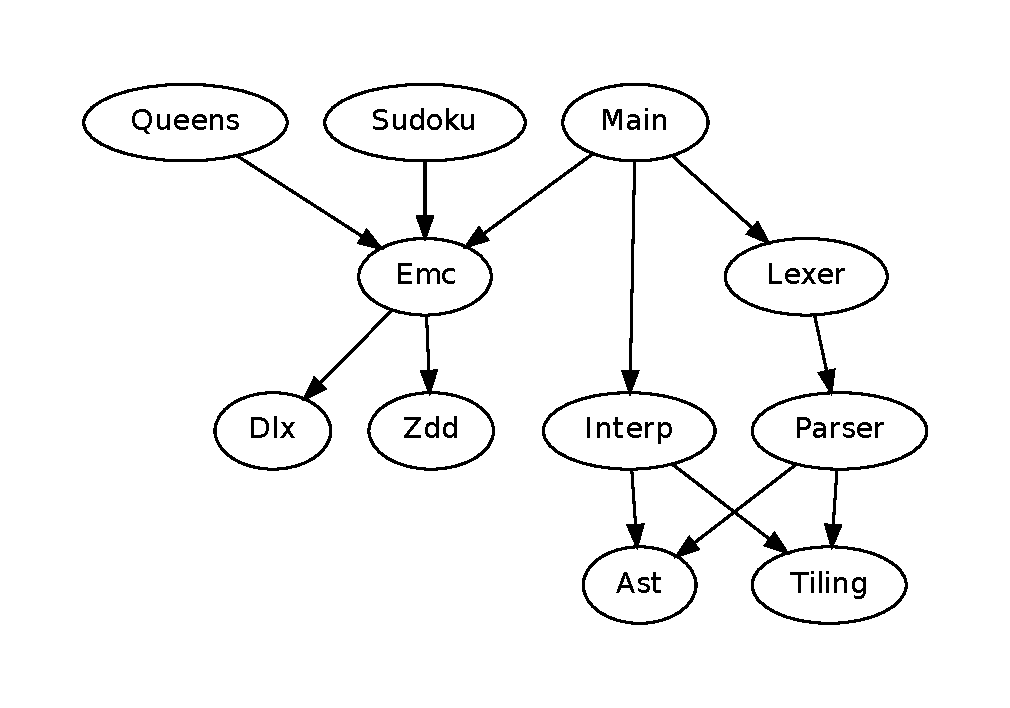
\includegraphics[scale=0.5]{../imports/archi.pdf}
\end{center}
\end{figure}
\end{frame}

\begin{frame}[fragile]{ReMl : Un mini langage pour le pavage}

Probleme sous forme de patterns : 
\begin{columns}
    \column{0.3\textwidth}
\begin{lstlisting}
pattern b = {
**
.*
**
}
\end{lstlisting}
    \column{0.1\textwidth}
		$\rightarrow$
    \column{0.3\textwidth}
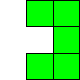
\includegraphics[scale=1]{../imports/patron.pdf}
\end{columns}
\end{frame}

\begin{frame}{ReMl : definir un problème}

\lstinputlisting[language=Caml]{../imports/non-regression.rem}

\#présence d'options :  
\emph{$\sim$sym}, "\emph{$\sim$one}" ou "\emph{$\sim$maybe}"
 
 \end{frame}


\begin{frame}{ReMl : les transformations}
 
\begin{description}
\item[Les positive] rotations $90\,^{\circ}$, $180\,^{\circ}$, 
$270\,^{\circ}$ et Identité
\item[Les négatives] Réflexion vertical, horizontale, première et 
deuxième diagonal
\end{description}
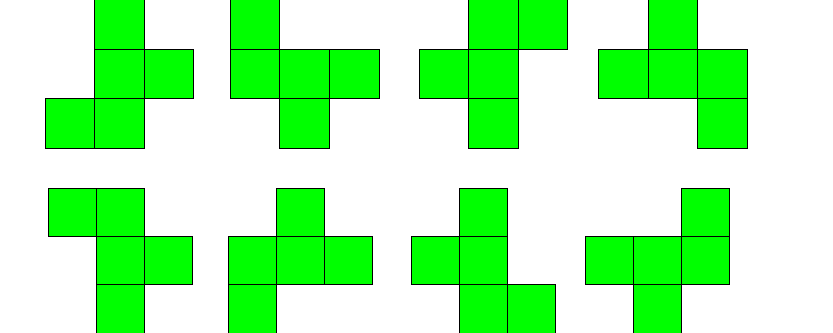
\includegraphics[scale=0.5]{../imports/transformations.pdf}
\end{frame}




\begin{frame}{Conclusion}

Résultats :  
\begin{itemize}
\item Des algoritmhes qui fonctionnent (résultats cohérent)
\item Une bibliothèque facile d'utilisation
\end{itemize}

 Aller plus loin : 
\begin{itemize}
\item Optimisations des calcules en fonction des symmétries du problème
\item Ajout de fonctionnalités dans le langage
\item Documentation
\end{itemize}



\end{frame}

\end{document}
